\documentclass[pdftex,12pt,a4paper]{report} 

% Document settings

\usepackage{fullpage}
\usepackage{cite}
\usepackage{datetime} 
\usepackage{geometry}
\usepackage[pdftex]{graphicx}
\usepackage{verbatim}
\usepackage{todonotes}
\usepackage{array}
\usepackage{capt-of}
\usepackage[parfill]{parskip}
\usepackage{underscore}
\usepackage{url}
\usepackage{listings}


 \usepackage{courier}
 \lstset{
         basicstyle=\footnotesize\ttfamily, 
         numberstyle=\tiny,      
	language=Java,
 }
 \lstloadlanguages{
         Java
 }


\geometry{verbose,lmargin=3cm,rmargin=3cm}

\newcommand{\HRule}{\rule{\linewidth}{0.5mm}}

\begin{document}

\title{Computer Music Improvisation - A Grammatical Approach For Jazz/Blues}
\author{Cliff Sun (chs09)}
\date{June 2013}
\maketitle


\setcounter{tocdepth}{2} % Set the depth of toc indexing

\tableofcontents

\pagebreak

\renewcommand*\thesection{\arabic{section}}

% \section{Acknowledgements}

% acknowledge

\pagebreak

\chapter{Introduction}

\section{Motivation \& Overview}
Improvisation is often seen as a human activity, especially in the domain of music. Genre's such as Jazz and Blues are heavily based on the performer improvising on a set form. The art of improvisation can essentially be summarised to a set of skills and rules with accompanying music theory that needs to be learnt by the performer. In this regard, we can say that it is entirely possible that a computer can 'improvise'. However we can also argue that improvisation also involves creativity (as does any form of art), which is extremely much harder to describe. The aim of this project is to be able to model and replicate such music improvisation using a computer. There have been many different approaches for melody generation/improvisation in blues and jazz over the years and many of them have involved a statistical/machine learning approach. We explore a more grammatical approach which uses an abstract musical grammar which will allow us to create well-defined structures and rhythms for jazz melodies. The area of computational creativity in music has been explored before and is still ongoing, and we hope that this project can provide a new approach for computer music improvisation. 


\paragraph{Improvisation vs Composition}
Music improvisation can be defined as the creative activity of immediate composition, or 'Composition on the fly'. In the case of this project, both terms will be used interchangeably.

\section{Project Domain - Computational Creativity}
The project comes under the area of computational creativity, and it's immediate uses and contributions are fairly novel. We could say that one of the main challenges of computational creativity is to encapsulate the creative processes of a human being into a computer. This is a non-trivial task as such, the human brain is an extremely complicated entity with which we still do not have a full understanding of and thus it is difficult to define what creativity objectively means. On the other hand, computational creativity can also help us understand further the behaviour of creativity in humans. As a result, a project in the field of computational creativity is often very experimental in terms of its approach and it's end result. 

Much work has been done in the field of generated visual art with tools and programs such as Simon Colton's Painting Fool \cite{website:paintingfool} and Harold Cohen's AARON \cite{website:aaron} both of which create original artistic images to a high standard.

Evaluation of such projects is not easy, usually such projects will produce an output of an artistic form (music/art/literature) and as such evaluation can be very subjective depending on the person. The best way to evaluate the result of such a project (in terms of music) would be to do a turing test to compare a similar human composed piece of music to the output of the new program. We can score the program and its output based on whether the listener can or can not identify which piece of music was compose by a computer and which was composed by a human. This will be explained more in the Evaluation section.

\section{Related Works}
Work on computer music improvisation dates back 20-30 years or so. One famous example of computer generated music in general is David Cope's EMI (Experiments in Music Intelligence) which produces music in the style of various composers (using existing works as input sources). In terms of computer improvisation for jazz and blues music, there have been numerous machine learning approaches. One such piece of work is entitled 'Finding temporal structure in music: Blues improvisation with LSTM recurrent networks' By Eck and Schmidhuber (2002) \cite{eck02}. In addition Belinda Thom's Band-out-of-a-Box (BoB) describes an interactive soloist which can improvise with another performer using unsupervised learning in 'Unsupervised Learning and Interactive Jazz/Blues Improvisation' (2000) \cite{thom2000}.

Other works regarding grammatical approaches for music improvisation include approaches based on string rewriting grammars (L-systems) in 'Grammar Based Music Composition' by McCormack (1996) \cite{mccormack96}. In addition 'A Grammatical Approach to Automatic Improvisation' by Keller and Madison \cite{keller07} introduces a formal grammar for music improvisation in which we will be basing our work on (see more below).

In addition and in relation to Keller's above mentioned paper \cite{keller07} we also note that work has also been done by Keller to learn jazz grammars from a corpus of jazz melodies. Learning Jazz Grammars by Gillick, Tang and Keller \cite{kellergillick09} uses a machine learning approach (combining clustering and markov chains) to learn abstract grammars which can be used to produce jazz melodies (using the same system that \cite{keller07} produces). 


\pagebreak

\chapter{Background - Musical Theory}


\section{Blues Improvisation}
Blues is one of the most common genres that relies on performer improvisation. Performers of this genre tend to play a musical instrument (including voice) on top of an accompaniment with a well defined structure/form. The blues form itself is often defined by its 12 bar chord progression (commonly called 12 bar blues) which is essentially a standard harmonic chord progression of 12 bars in a standard 4/4 time signature. Table 1.1 below shows the chords for the general 12 bar blues form, with I7 referring to the harmonic seventh Tonic chord. Chord IV refers to the 'dominant' chord (4th degree) and Chord V refers to the 'dominant' chord (4th degree).


\begin{table}[here]
\centering
\newcolumntype{C}{>{\centering\arraybackslash}m{23pt}<{}}
\begin{tabular}{|*{12}{C|}}
  I & I or IV & I & I7 & IV & IV & I & I7 & V & V or IV & I & I or V
\end{tabular}
\caption{12 bar blues chord progressions}
\label{12 bar blues}
\end{table}


\begin{table}[here]
\centering
\newcolumntype{C}{>{\centering\arraybackslash}m{23pt}<{}}
\begin{tabular}{|*{12}{C|}}
  I & I & I & I & IV & IV & I & I & V & IV & I & I
\end{tabular}
\caption{12 bar blues simplified chord progression}
\label{12 bar blues}
\end{table}


Table 1.2 gives us one possible (and simple) chord progression for 12 bar blues in which we will basing our improvisation upon. 


\subsection{Blue Notes} What really gives the blues genre it's characteristics are the 'blue notes'. These are notes which are played at a lower pitch (flatter) than that of the major scale (usually one semitone lower on piano). The notes which are 'flattened' are the \textbf{third}, \textbf{fifth} and \textbf{seventh} notes of the major scale.
There are theoretical reasons for the introduction of 'blue notes' which we won't go into detail here. But essentially these 'blue notes' allow for moments of expression in blues melodies. 

\subsection{Blues and Pentatonic Scales}
Blues scales include the blue notes that we've mentioned above, these scales give the performer a set of notes to improvise with and gives the music the characteristic 'blues' feel to it. Blues scales are generally based on the major/minor pentatonic scale. A pentatonic scale is a scale of five notes (compared to seven notes in regular major/minor scale) and is widely used in music across the world. The most common blues scale (and the one we are going to be basing our improvisations on) is the blues minor scale which is based on the minor pentatonic scale (see Figure \ref{fig:cminorpentatonicscale}) with a sharp 4th note (or a flat 5th note, both are equivalent). In Figure \ref{fig:cminorbluesscale} we can see the blues minor scale includes all the blue notes; E(3rd degree) flat, G(5th degree) flat and B(7th degree) flat.

\begin{figure}[here]
  \centering
  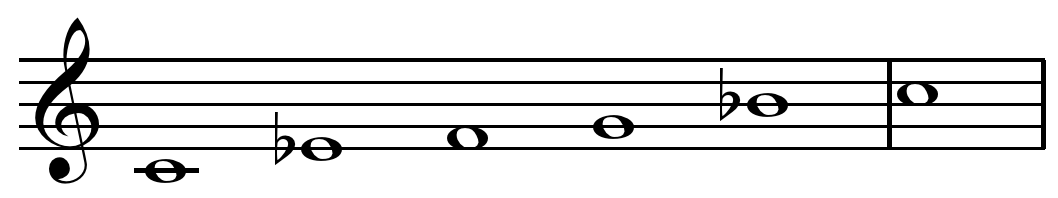
\includegraphics[scale=0.3]{figure/minorpentatonicscale.png}
  \captionof{figure}{C minor pentatonic scale}
  \label{fig:cminorpentatonicscale}
\end{figure}

\begin{figure}[here]
  \centering
  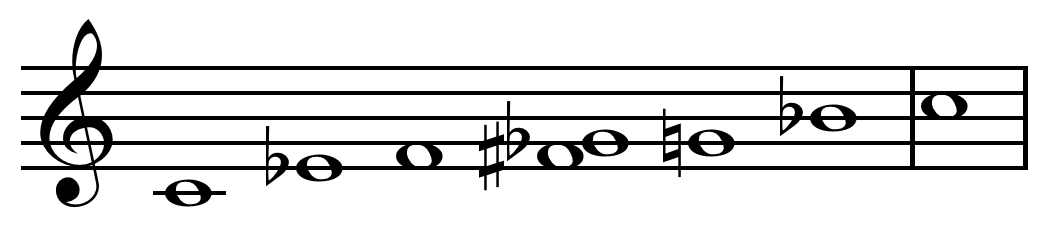
\includegraphics[scale=0.3]{figure/bluesminorhexatonicscale.png}
  \captionof{figure}{C minor blues (hexatonic) scale}
  \label{fig:cminorbluesscale}
\end{figure}

\section{Jazz Improvisation}

\subsection{Versus Blues}
Though it is common to use terms blues and jazz interchangeably, the reality is that they are very much different styles of music. However it is very difficult to categorise these two genres of music and much of the genre is overlapping. We'll refer to our music as fitting both jazz and blues during this report.

Blues itself has a very simplistic style, it relies on basic chord progressions (I IV V as we've seen above) which are repeated over and over again. By using one scale (pentatonic or minor blues scale) we can easily improvise a melody on top of the progression. In addition feeling and emotion is important in blues music and thus blues is based more on expression rather than technical ability. 

Jazz has many roots in blues music (in fact the blues from is ubiquitous in jazz music), the 12 bar progression is commonly used in Jazz music in addition to blue notes for expressive purposes. However Jazz itself is much more complex than blues and uses many more chords/scales, time signatures and melodic structures than blues. For example Jazz's rhythms tend to use syncopation (playing on the off beat) and swung notes i.e. playing two notes (which have the same duration) with different durations, where the first note has the longer duration and the second one the shorter. In addition Jazz chord theory itself is a very complicated as we shall see below.

\section{Basic Jazz Theory}
Jazz theory is extremely comprehensive and reflects in the complexity and the range of the music that belongs to this genre. Books such as 'The Jazz Piano Book' by Mark Levine provide a comprehensive learning guide to aid and teach jazz pianists the complex chord theory that jazz imposes. As it covers almost everything a beginner/intermediate jazz pianist needs to know to be able to improvise/play jazz, we will not go into it here. But we will highlight some of the more relevant ideas that we are using in our project.

\subsection{Chord Voicings}
Often a good way to start/learn simple jazz improvisation is to learn jazz chord voicings, these are essentially accompanying chords in the left hand which allows the pianist to use their right hand to play the melody and improvise. Chord extensions can be used to provide variations in the left hand voicings, for example adding the sixth, ninth and thirteenth scale note to the chord. Various progressions can be constructed using the large vocabulary of chord voicings, though many are based on the same underlying basic progression.

\subsection{Chord Substitution}
Chord substitutions are very common in Jazz, where a player/composer would use a chord in place of another related chord. Often it is just changing a note or two in the chord, but this small change often creates variety and interest and is what gives jazz music it's harmonic and melodic variety. The theory behind this is fairly complex and we won't be exploring this further, but the idea is that chord substitutions are possible and allow a richer variety in the music.

\subsection{Scale Theory - Playing Off the Chord}
As explained previously chord voicings allow us to have a varied left hand accompaniment which allows the right hand to improvise melodies. One simple way we can improvise melodies is to use scales that fit with the chord voicings. Indeed much of jazz is based on playing over the chords and being able to follow the chord changes itself. Certain scales fit different chords and thus it is up to the performer to choose the right scale to use to improvise a melody. Note that when we talk about scales here we do not mean in terms of sequence of notes, but rather the collection of notes that belong to the scale.

\subsubsection{Scales \& Modes}
For a simplified example, we can say that in the key of C major, the C major scale can be used over the II, V and I chord, i.e. Dm(7), G(7) and C. This is because for each chord, the 3rd and 7th note exists in the C major scale. We've discussed previously that the 3rd and 7th of a chord and scale indicates/identifies the tonality of the chord and scale. Thus it is reasonable to point out that scales with the same 3rd and 7th as a chord can be used to improvise on top of the chord.
If we look at it from another approach, then we can say that the chords used (and the tonality of the chords, i.e. major/minor/dominant) for the progression can be derived directly from the C major scale itself. To do this we must introduce an important piece of musical theory called modes. A mode is essentially a scale that can start from anywhere (not just the tonic C). There are 7 different modes in C major, each mode (scale) starting from a different note in the C major scale, below is an example of the 7 modes in C major and their corresponding names  \cite{jazzmusicmakers}.

\begin{figure}[here]
  \centering
  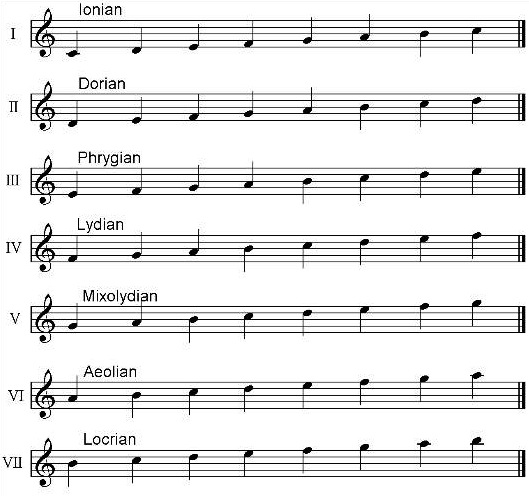
\includegraphics[scale=2.7]{figure/cmajormodes.jpg}
  \captionof{figure}{Modes for the C major scale}
  \label{fig:cmajormodes}
\end{figure}

If we look at the second (Dorian) mode we see that it starts from D and has an F natural and a C natural (3rd and 7th note respectively). This does not correspond to any D major/minor scale, which gives us the reason for having modes (allowing us to express and formalise different sequences of notes). If we take the 1st, 3rd and 7th of the Dorian mode, we get a D minor 7th chord (D, F, C), i.e. the II chord in our above progression. Similarly, if we take the fifth (Mixolydian) mode which starts from G, and we take the 1st, 3rd and 7th notes, we end up with a G dominant 7th chord (G, B, F). C major Ionian mode is trivial and thus we have our basic II-V-I progression derived from C major and it's modes. 
These modes also point out to us the avoid notes for each chord. The avoid note generally tends to be the 4th note, i.e. for the G7 chord, we use the fifth (Mixolydian) mode, where the C is the avoid note. This is because if you were to play a C on top of the G7 chord, it would sound dissonant. But avoid notes themselves can be used as passing notes where they don't have as much of a tonal impact in the music. As such, when we are in the key of C major and we have a dominant seventh chord in our left hand (G7), we can use the Mixolydian scale to improvise on top of the G7 chord. The above theory constitutes Major scale harmonies. It is also possible to 'raise' the 4th note (augmented, annotated as +4) as an alternate to having the 'avoid' note. For example we may use the first mode in C major (Ionian) and raise the 4th (F natural) to F sharp. We can see the effect of this \ref{fig:clydian} taken from the Jazz Piano Book. In effect we have changed the key and as such the key happens to be G major. This means the new scale is in fact the C Lydian mode (in G major). However raising the 4th does not always in effect give us a new mode which corresponds to a different (major) key. Sometimes the new scale does not match any major key but rather is based on melodic minor scales. This brings us to Melodic Minor scale harmonies, however we won't go into this further, but it is important to realise the complexity of scales and scale theory not only for jazz, but for music in general.

\begin{figure}[here]
  \centering
  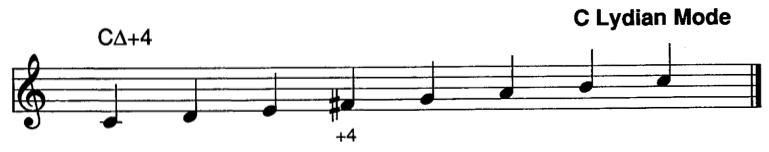
\includegraphics[scale=0.45]{figure/clydian.png}
  \captionof{figure}{C Lydian mode (in the key of G major)}
  \label{fig:clydian}
\end{figure}

Note in summary that it is important to think about the key that we are playing in, rather than the specific chord. We may end up using scales that are actually modes in alternative keys, which gives us musical variety in the improvisations.

The different scales and modes that we can use provide us with alternative scales to use for improvisation over  different jazz voicings thus allowing for variety in the music. In our case we intend to represent this as best as we can whilst keeping it simple to ensure that our problem domain does not become too complicated.

\section{Computer Improvisation For Blues/Jazz}

\subsection{Overview}
The idea behind jazz improvisation on the computer is that whilst jazz is essentially composition during performance (composition concurrent/on the fly), the composition is not completely done on the spot. Jazz musicians will practice many jazz licks, voicing's and scales before hand so that they can go into a performance with the required knowledge and practice needed to improvise jazz. Blues is also similar, blues musicians will practice pentatonic and minor blues scales whilst learning blues/jazz licks. Prior knowledge (knowledge of chord and scale theory) is a definite requirement in order be able to improvise blues/jazz at an advanced level.

\subsection{Difficulty/Complexity}
Blues and jazz music can range from something extremely simple such as playing the minor blues / pentatonic scale over a variation of the 12 bar blues progression, to complex theory involving left hand voicings, chord substitutions (tritone substitutions for example) and scale theory (and scale modes such as Ionian, Lydian, Mixolydian etc). Our aim is to be able to incorporate and encapsulate as much jazz theory as we can in the system that we are developing such that it can produce music with vast melodic and harmonic variations. Strictly speaking, the music that we generate may not strongly adhere to either a blues/jazz style (i.e. it may not easily identified with a jazz sub-genre or with a famous jazz musician) but is rather based on the ideas of blues and jazz improvisation. In addition the aim is to be able to provide a general solution that does not just produce a limited style and sound but rather be able to improvise a melody on any chord progression that we can give it. As a starting point, our goal is to generate/improvise jazz blues melodies on top of a 12 bar progression using a computer. Musical improvisation also covers improvisation/variations for the accompaniment as well. A grammar for comprehensive chord substitutions in improvising accompaniments in 12 bar blues/jazz is covered in Steedman's paper 'The Blues and the Abstract Truth: Music and Mental Models' \cite{steedman96}. However in this project our main focus is on melody generation.

Due to the project's time constraints and the complexity of jazz music, we are only aiming to be able to produce something that improvises jazz music to a beginner/intermediate level. The main challenge behind this project is the experimentation and uncertainty of using a grammatical approach to improvise music. Having a more realistic/achievable target (producing beginner's level jazz music) we have simplified the overall problem which allow us to concentrate on the technical aspect of the project.

\paragraph{Keys}
It is well known that the characteristic of music i.e. the listening experience is not based on the pitches of each note, but the pitch changes between each note. Thus a melody played in different keys will be recognisable to any listener familiar with the melody. For this reason we can simplify our problem further by working (melody generations/chord progressions) in the same key, the key of C. We will be basing improvisations on the C minor 7th scale and use a simplified 12 bar blues/jazz progression in the key of C.


\pagebreak

\chapter{Background - Grammar For Blues}

\section{Introduction}
In this project we propose a grammatical approach for generating blues melodies. Grammars have been used in other works in the field of computer music improvisation (see Chapter 1 - Related Works). More dominant however is the use of machine learning techniques for music improvisation/generation. 'Finding temporal structure in music: Blues improvisation with LSTM recurrent networks' By Eck and Schmidhuber (2002) \cite{eck02} is a more recent example of using LSTM networks to generate blues melodies. However there is a need for a training set and the result is affected by the quality of the training set. Using a grammar means that we don't need to encode a training set or input set and can directly influence our resulting sound.

\section{Grammars and Music}
Grammars enforce structures within music and such a linguistic approach seems suitable for the 'call and response' nature of African-American influenced music such as blues. We can compare a line of melody to a sentence in natural language. For example a sequence of notes and the rhythm that they occur in gives a melody it's own character and meaning, like a sentence in natural language. However in music there are no semantic rules in terms of the melody, it is entirely up to the listener/player as to how they interpret it. This is where a grammar comes in, grammars are structural rules that govern the composition of 'sentences' (in the case of natural language) and such grammars are not concerned with the semantics of the sentence. Therefore a well-defined grammar for blues music should be able to produce well-structured blues melodies.


\section{Initial Non-Grammatical Approach}
Before diving into a grammatical approach for blues melody improvisations, we decided to explore some simple ideas regarding probabilistic generation of notes in a sequence. Below are two simple approaches that we took. Note that we could easily classify these approaches with a simple grammar, however the point of introducing a grammar is so that we can defined structure and rhythm in our melodies, so for now we say that the first two simple approaches/implementations are not a 'grammatical' approach.

\subsection{Simple Probabilistic Generation (with fixed duration)}
We decided to make a quick music improvisation tool which uses probabilities to pick the next note in the melody. We kept the duration constant (a quaver/eighth note) and kept the range within one octave. An example of the generation is shown below in Figure \ref{fig:randomgeneration}. We designed it so that the probability that we choose the next note has an inverse relation to the interval of the note itself. I.e. the probability is of choosing an adjacent note in the blues scale is highest, with the probability for choosing a note that is 2 notes apart lower. In addition we made it so that the probability that we choose a note so that sequence is going in the same direction is higher than choosing a note that changes the direction of the sequence. For example if we had an F (natural) followed by an F\#, the probability of choosing G is higher than choosing an F (natural) (both one note interval from F\#).

\begin{figure}[here]
  \centering
  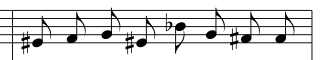
\includegraphics[scale=0.7]{figure/randomgeneration.png}
  \captionof{figure}{Probabilistic generation for a blues sequence}
  \label{fig:probabilisticgeneration}
\end{figure}

In the figure above we can see that a probabilistic random generation of notes with some constraints yields a fairly decent result. The notes are all part of the blues scale and so sound acceptable as a blues melody, however it lacks structure and rhythm as all the notes are of the same duration. 

\subsection{Probabilistic Generation With Mixed Durations}
To add some rhythm to the melody we decided that we could randomly choose duration lengths when we chose the next note. In our implementation we limited ourselves to semiquaver (16th), quaver (8th), and crotchet (quarter) notes. The idea was to introduce some style of rhythm to the music in the hopes of trying to make the melody fit into the blues criteria.

In Figure \ref{fig:randomgenerationwithdifferentdurations} we can see that choosing a random duration can give decent results. In our case we have an example of syncopation with the Eb quaver being played half a beat after the second beat. This sounds interesting and much more like blues music than in the previous example (in section 3.1). However not all bars generated look like this, some don't sound pleasing at all and some sound wrong rhythmically. As we are generating random durations, we are generating random rhythms and sequences and we may occasionally get a good melody, but a lot of the time we get bad or awkward rhythms. 

\begin{figure}[here]
  \centering
  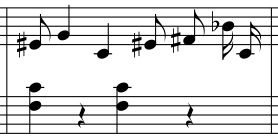
\includegraphics[scale=0.6]{figure/randomgenerationdifferentdurations.png}
  \captionof{figure}{Probabilistic generation with varying durations}
  \label{fig:probabilisticgenerationwithdifferentdurations}
\end{figure}


\section{Adding a Grammar For Blues}
The initial approaches are promising and give us a good foundation to build upon. If we randomly choose notes from a blues scale, they generally sound acceptable/good in terms of the pitch. However we have identified that some of the melodies/bars do not sound good rhythmically, i.e. they either don't sound good at all, or don't have the blues characteristics. We can see now that the rhythm of the notes is just as important as the pitch of the notes. 

In Keller and Madison's paper \cite{keller07}, a comprehensive grammar for blues is specified with excellent results. In particular a stochastic context-free grammar is used, where production rules of a context-free grammar are augmented with a probability/weighting. By using ideas from this approach we hope that we can create a more comprehensive grammar with more scope for variations. The terminal alphabet for the grammar is classified into different types of 'tones'. A grammar can use these different types of tones to form a melodic sequence. The classification of different tones is very much applicable to blues/jazz improvisation where knowledge of how to put these different types of tones together mean a better sounding melody is formed. In our previous non-grammatical examples, we use only notes from the blues scale. Though they sounded fine musically, using such a small set of notes means that the melody sounds flat and uninteresting for the most part. It is actually valid in music to use notes that aren't part of the scale, they can be used as a 'passing note' for example and as such makes the melody sound more interesting and complete. An article by Keller entitled 'How to Improvise Jazz Melodies' \cite{jazzkeller} talks about different methods for improvising blues/jazz melodies. The article provides many different methods and guidelines for improvising jazz/blues melodies. The above mentioned paper \cite{keller07} however only uses a few of these guidelines (albeit the most important ones). The classification of notes/tones are as follows:

\begin{description}
  \item[Chord Tones (\textit{C})] are tones (notes) which belong to the current chord we are improvising on top of.
  \item[Colour Tones (\textit{L})] are auxiliary tones for the current chord which sound correct musically when played with the current chord as an accompaniment. In particular, colour tones do not belong to the notes in the chord. 
  \item[Approach Tones (\textit{A})] are also notes which aren't in the chord (not the same as colour tones either) but they make good transitions to chord-tones or colour tones. These are also sometimes known as 'passing notes' where such a note can be placed between two chord/colours to make the melody seemed less disjointed. It is often bad practice however to place two approach tones next to each other.
  \item[Other] tones which don't belong to any of the above. These may include a rest \textbf{(\textit{R})}, or a scale tone \textbf{(\textit{S})} (a tone in the scale which works musically with the accompanying chord).
\end{description}

The issue we were concerned with before was whether we should deal with pitches of notes separately from the duration of the note. We have an option to create a grammar just for the rhythm of the melodic sequence. However randomly picking notes from the scale will not give us a result as good as the one in Keller and Madison 2007. The idea of chord, colour and approach tones provides us with a much better method of generating better sounding melodies.

\subsection{Context-Free Grammars}
The grammar described above is a context-free grammar. A grammar is considered context-free if the rules (production rules) of the grammar can be applied, i.e. the non-terminals can be written, without being dependant on the surrounding symbols. The majority of natural languages can be said to be based on context-free grammars. In addition we can say that the implementation of such a grammar for blues music is similar (and should be similar) to the implementation style of context-free grammars for random sentence generators. 

Context-free grammars are defined by the 4-tuple (V,$\Sigma$,R,S):

\begin{description}
  \item[V] - a finite set of \emph{variables}(non-terminal characters). Each variable essentially represents a different way to put together different families of notes and durations.
  \item[$\Sigma$]  - a finite set of \emph{terminals} which contain the actual content. In the case of our grammar, the terminals represent the type of tones/notes in the sequence.
  \item[R] - a set of production \emph{rules} in the form of A $\rightarrow$ b, where A is a variable $\in$V and b could be a sequence of variables and/or terminals.
  \item[S] - the starting variable/symbol used to represent the whole sentences where S$\in$V.
\end{description}


We start with starting variable S and expand the right hand side of the rule for S using other production rules. Expansion occurs by replacing variables in the sequence with the right hand side of the rule for that variable. We do this until the final result is a sequence of terminals only.

\subsubsection{Stochastic Context-Free Grammar}
The grammar that is defined in Keller's paper \cite{keller07} is a context-free grammar with probabilities, a stochastic/probabilistic context-free grammar. Each production rule has a probability associated with it which determines the likelihood of which production rule to use (if there are more than 1 with the same variable on the left hand side). The grammar specified below is such a grammar.

\subsection{Blues Grammar}
We aim to implement the grammar described in the paper by Keller \cite{keller07} and extend it or make improvements to it. The grammar itself is essentially a set of production rules which represent different rhythmic phrases with families of tones and their duration as the terminals. At the top level, we have the production rules P(n) $\rightarrow$ ... where n is the length of the melody generated in quarter/crotchet beats and n $\in$ 1..N:

\begin{verbatim}


P(0) -> empty [1]
P(1) -> Q1 [1] 
P(2) -> Q2 [1] 
P(3) -> Q2 Q1 [1] 
P(n) -> Q1 P(n−1)  [ .4 ]
P(n) -> Q2 P(n−2)  [ .4 ] 
P(n) -> Q4 P(n−4)  [ .2 ]

\end{verbatim}

A P variable takes in argument n, which limits the generation of the melody to fit n beats. We could also have a recursive grammar which expands until it reaches a set limit, but we may end up truncating a phrase which is not preferred. The values in the square brackets denote the weights for choosing a particular rule. It is worth noting that for the rules above, the weights are the same as probabilities (they add up to 1, so for P(n):  0.4+0.4+0.2 = 1), however it is not a requirement. The weights will will be normalised so that the actual probabilities are worked out.

The rest of the rules are taken from the aforementioned paper. We have rewritten the names of variables so that the numbers which follow a letter (i.e. Q4, V1, N/2 etc) denote the length of the notes generated (in quarter/crotchet beats). For example all the terminal sequences that can be generated from variable Q4 will have a total length of 4 crotchet beats. In addition, the number of beats that V/2 produces is half a beat (and also any other variable with /2). The specification of the grammar in Keller's paper \cite{keller07} is slightly inconsistent in the variable naming convention and can cause confusion. Therefore the rules (with new renamed variables) are as follows:

\begin{verbatim}


Q4 -> Q2 V1 V1  [0.52]
Q4 -> V/2 N1 N1 N1 V/2  [0.01]
Q4 -> V1 Q2 V1  [0.47]

Q2 -> N2  [0.06]
Q2 -> V1 V1  [0.6]
Q2 -> V/2 N1 V/2  [0.12]
Q2 -> H3/2 N/2  [0.16]
Q2 -> ({3} H1 H1 H1)  [0.06]

Q1 -> C1  [1]

V1 -> N1  [0.22]
V1 -> V/2 V/2  [0.72]
V1 -> ({3} H/2 H/2 H/2)  [0.05]
V1 -> ({3} H/2 H/2 A/2)  [0.01]

V/2 -> N/2  [0.99]
V/2 -> H/4 A/4  [0.01]

N2 -> C2  [1]

N1 -> C1  [0.5]
N1 -> L1  [0.2]
N1 -> S1  [0.5]
N1 -> A1  [0.01]
N1 -> R1  [0.25]
N/2 -> C/2  [0.4]
N/2 -> L/2  [0.2]
N/2 -> S/2  [0.4]
N/2 -> A/2  [0.01]
N/2 -> R/2  [0.1]

\end{verbatim}

In the N-variables, C, L, S, A and R are terminals in the terminal alphabet. They are shorthand for the families of tones that we've described at the beginning of the section. The grammar itself contains 4 distinct levels / types of variables:

\begin{description}
  \item[N-variables] - e.g. N2, N1 and N/2. These variables are at the bottom of the tree and their rule is always rewritten as a single terminal with the same length as the variable (see above).
  \item[V-variables]  - e.g. V1 and V/2. These are intermediate variables that describe small rhythmic sections. They allow the specification of different ways of making up a certain number of beats. For example we could add rules for V1 to represent more possible phrases, such as [V1 $\rightarrow$ H/4 N/2 H/4] if we wanted to add more variety to the music. They use the N-variables above to construct the sections. Note that the H-variable is a terminal which represents a \textbf{helpful} tone and refers to any of the Chord (\textit{C}), Colour (\textit{L}) and Approach (\textit{A}) tones.
  \item[Q-variables] - e.g. Q4, Q2, Q1. These are top level variables which essentially combine smaller sections/phrases to produce the larger sections. 
  \item[P-variable] - e.g P(n), the starting variable (as seen previously).
\end{description}

Again each rule has a probability associated with it and the above probabilities are taken from the above mentioned paper. The probabilities themselves play a large role in how the resulting melody sounds and at the moment can only be adjusted by the user.

Each unique derivation for each duration we generate for (the n in the P(n) starting variable) has its own unique parse tree. Figure \ref{fig:Q2parsetree} shows a partial parse tree just for Q2, which is already fairly comprehensive. We can see that the overall probability for generating a terminal sequence \emph{C1 C1} or \emph{C1 S1} from Q2 is 0.6x0.22*0.22*0.34*0.34= 0.00336. It is worth noting that many more melodies can be created with one particular terminal sequence, which we will discuss below.

The implementation of the above grammar will give the same results as in Keller's paper \cite{keller07}, indeed changes and enhancements may be made along the way to try and improve the result. 
It would also be better if we could allow users to adjust the grammar themselves to produce different melodies, for example a more complex grammar would perhaps produce a more complex melody. 

\begin{figure}[here]
  \centering
  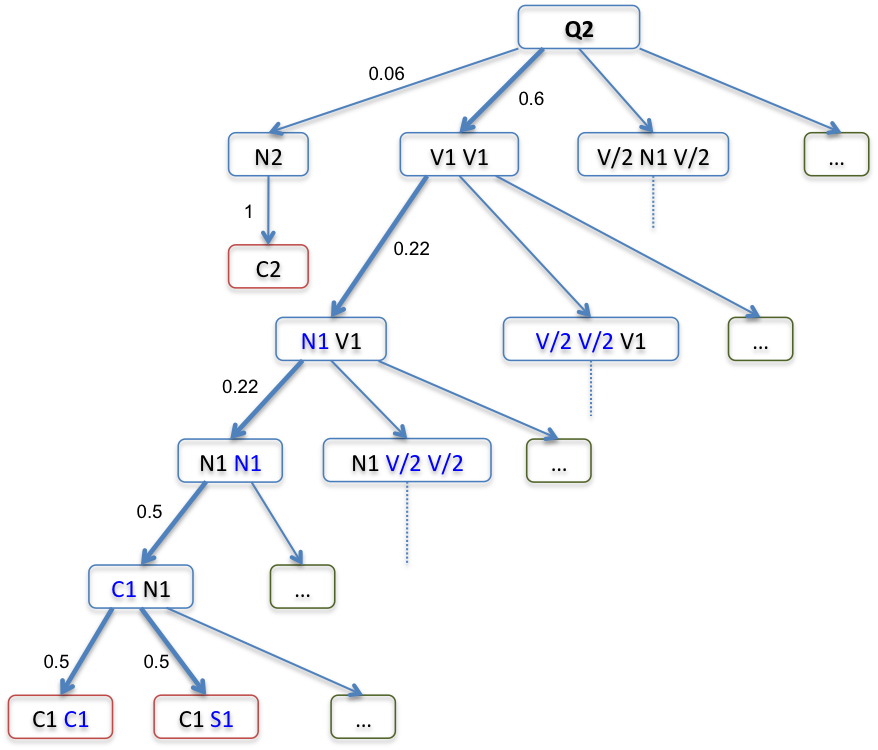
\includegraphics[scale=0.8]{figure/Q2parsetree.png}
  \captionof{figure}{Parse tree for Q2}
  \label{fig:Q2parsetree}
\end{figure}

\subsection{Terminal Sequences to Melodic Sequences}
As we've discussed previously, the grammar above generates a terminal sequence of types of tones and durations. Additional work needs to be done in order to produce a sequence of actual musical notes. An example terminal sequence that may be generated for P(4) $\rightarrow$ Q2 Q2 may be:

\begin{verbatim}
C/2 L1 H/4 A/4 H3/2 S/2
\end{verbatim}

We could generate many melodic sequences from the terminal sequence alone. However we would prefer to generate better sound melodies if possible. To do this we would have to introduce constraints when choosing actual musical notes from the families of tones, otherwise we may end up with a melody that sounds as random as our non-grammatical attempts. To do this we refer to Keller's article 'How to Improvise Jazz Melodies' \cite{jazzkeller}. Here are some possible ways we can constrain the selection of notes to ensure a better sounding melody:

\begin{description}
  \item[Know scales that go off the chords] scale here refers to a set of notes, rather than a sequence. If we know what scale works for the current chord, then it can help constrain the choice of tones so that the melody is closer to the scale.
  \item[Intervals between notes] smaller intervals often sound more pleasing than large intervals, however it is good to have both. If our intervals are too big then the melody will sound quite discordant. However alternatively 'skipping' notes can sound good if combined with a direction change (see below) and can give a zig-zagged effect.
  \item[Change direction] if we have a sequence of small intervals (scale-like sequence) we may want to change direction at some point to provide variety and make the melody sound more interesting. We don't want to do this too often however as it may sound disorientating.
  \item[Use of enclosures] similar to direction changes, we can approach a note from both sides alternatively. This involves making sure intervals get smaller and also direction changes occur. Enclosures work better if the target tone is a chord tone.
\end{description}

By implementing these musical features, we can avoid awkward note combinations and optimise the melodic sequence from the terminal sequence.


\chapter{Genetic/Evolutionary Algorithm Extension}

\section{Approach}
The problem with a grammar is that it has a finite search space, this is more noticeable with a smaller grammar. The music generated from the context free grammar in Chapter 2 will always resemble the same style and more importantly the same complexity. In reality, a human musician learns and continually improves over time, for example they may discover a new style to play music or find a new phrase/jazz lick that sounds better. They also improve their skills and  If we want our computer to be able to improvise like a human then we would need for it to 'evolve'.

The idea in this is that we would like to be able to allow our program to continue to produce 'new' music and improve on our improvisations/compositions. We can do this using evolutionary techniques such as selecting fragments/phrases from some melodies, then possibly add some sort of 'mutation' to it and recombining them together to form a new melody. The application of genetic algorithms may be useful for such a task. In particular interactive genetic algorithms, where the fitness function is the user or listener, due to the difficulty of judging musical quality computationally. However it may be possible to determine fitness based on simple melodic and rhythmic characteristics. 

Essentially we have to define our crossover function, our mutation function and our fitness function.

\section{Example}
A simple example would be show the user a selection of melodic sequences. The listener would indicate which sections sound good, or which sections sound bad (fitness function/evaluation). We can then perform crossovers of pairs of sequences to produce children. Crossovers could include swapping phrases around at the same place in the piece. We could then perform mutations on the child sequences such as altering the rhythm of a section. We would allow the fittest/best sounding sequences to be used more often for crossover, thereby producing better child sequences.

Crossover may also be done using terminal sequences (chord, colour approach tones etc) and not the actual sequence of notes. The reason for this is that swapping phrases of actual notes may result in disjointed sequences.

\chapter{Implementation}

\section{Overview}
The implementation of the blues improvisation using the grammar specified above will be primarily done in Java. Development will be done in the Eclipse IDE which provides good support including refactoring tools and auto-completion. Build management of the project is handled by Apache Maven, which manages dependencies and plugins required for the project. 

\section{Software Engineering Practices}
Software development is very much an iterative and incremental process. It is difficult to design the system correct on the first try and thus a lot of refactoring and changes may need to be done during the development process. In addition we hope that this piece of software forms a basis and platform upon which additional features can be implemented on top of. With both of these things in mind, it is important to make the system flexible and easy to extend. 

\section{Representation of Musical Score}
In order to make manipulating musical notes easier, we decided to write a seperate library (ABCJavaMusic) which allows us to represent musical notes/objects as java objects and represent/output them as ABC notation (see section 3.1). Although we could have used existing libraries and tools to represent our musical score, it is more beneficial overall to create a small/light-weight set of classes which do exactly what we want. This way, users can use this library to manipulate notes and scores and print them as ABC notation.

For example in Figure \ref{fig:abcnotationexample}, if we want to represent the notes as ABC notation (disregarding headers and bar lines in the ABC file) then it would look like:

\begin{verbatim}
C _D ^F3/2 _B,/2
\end{verbatim}

Where '$\_$' represents a flat, '$\wedge$' represents a sharp, and the ',' represents a lower octave. The duration of the note (in this case in quarter/crotchet beats) is the number directly after the pitch of the note (C, D, E all have a duration of 1 quarter beat). So F\# and B both have /2 which indicates the duration is half of a quarter/crotchet beat, i.e. an eighth/quaver.

In Java, we would represent these notes by writing this code:

\begin{lstlisting}
MainNoteComponent middleCNote = 
      new MainNoteComponent(BasicNote.C);
TimedComponent middleCNoteQuarter = 
      new TimedComponent(middleCNote, Duration.quarter);

MainNoteComponent DFlatNote = 
      new MainNoteComponent(BasicNote.D, AccidentalShift.Flat);
TimedComponent DFlatNoteQuarter = 
      new TimedComponent(DFlatAboveMiddleCNote, Duration.quarter);

MainNoteComponent FSharpNote = 
      new MainNoteComponent(BasicNote.F, AccidentalShift.Sharp);
TimedComponent FSharpNoteDottedQuarter = 
      new TimedComponent(FSharpNote, Duration.dottedQuarter);

MainNoteComponent BFlatBelowMiddleCNote = 
      new MainNoteComponent(BasicNote.B, AccidentalShift.Flat, -1);
TimedComponent BFlatBelowMiddleCNoteEighth = 
      new TimedComponent(BFlatBelowMiddleCNote, Duration.eighth);

\end{lstlisting}

To represent a bar with those notes (all in one phrase), we would write:

\begin{lstlisting}
Bar bar = new Bar();
StandardTimedComponentPhrase phrase = 
      new StandardTimedComponentPhrase();
phrase.addtoComponentList(middleCNoteQuarter);
phrase.addtoComponentList(DFlatNoteQuarter);
phrase.addtoComponentList(FSharpNoteDottedQuarter);
phrase.addtoComponentList(BFlatBelowMiddleCNoteEighth);
bar.addToBar(phrase);

\end{lstlisting}

By calling bar.getAbcRepresentation() we would get the abc representation of these notes as seen above. The representation is very verbose, however it is not intended to be used to represent complete pieces of music. ABC notation is designed for the actual music representation. For example in our system, we use the library to convert the terminal sequence from our grammar (sequences of Tones) to actual musical notes, using heuristics / probabilistic methods. 

\begin{figure}[here]
  \centering
  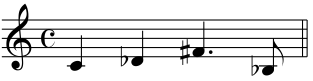
\includegraphics[scale=0.6]{figure/abcnotationexample.png}
  \captionof{figure}{Notes C, Dflat, Fsharp and Bflat}
  \label{fig:abcnotationexample}
\end{figure}

\subsection{ABC Notation}
ABC notation is a text-based music notation system which allows simple representation of musical scores. It is widely used in folk and traditional music and is ASCII based. There is support for the format including tools to convert abc notation to midi and to printable scores (as pdf's). More about the notation can be read on the website \url{abcnotation.com}.

\section{Grammar Implementation}
Numerous options have been explored for implementing the grammar (along with generation of melodic sequences) in Chapter 2, section 3.2. The main options are:

\begin{description}
  \item[Parser Generator Tools] such as ANTLR, which allows a context-free grammar to be specified using Extended Backus Naur Form and can generate lexers and parsers. It's main use is for generating a recogniser for a language define by the context-free grammar which checks the syntax of the input (a sample program in the specified language). ANTLR also has a maven plugin which can manage compilation of grammars.
  \item[External Languages] such as Python, or Lisp. These dynamic languages are useful for specifying a context-free grammar and generating sentences/sequences from the grammar. In particular in Lisp, a grammar can conveniently be expressed using s-expressions, a notation to represent a nested list hierarchy. Similarly a grammar can be represented using dictionaries in Python. Python has parsing libraries which can be used to create a parser and lexer for the inputted grammar file.
  \item[Native Implementation in Java] would keep the codebase all in one language. The implementation of the grammar may not be as straightforward as in Python or Lisp as we would have to represent everything as objects in Java. This approach is feasible if the grammar is small. However if we were to expand the grammar in the future then this may not be the best option.
\end{description}

We decided in the end to use Python parse the input grammar and to do sequence generation. Python is currently preferred due to existing experience and also the functional aspects of Python are ideal for sentence generation from a tree. As we want to be able to use both Java and Python together, we can use Jython, an implementation of Python written in Java (i.e. it runs on the JVM). This way we can invoke Python code from Java, allowing us to store our specified grammar in Python and invoke Python methods to generate sequences from the grammar. 
In terms of parsing the grammar, we used the PyParsing library, which allow us to represent the grammar to parse the musical grammar. 

\chapter{Evaluation}

\section{Overview}
We hope that the project can contribute something towards the field of creative music improvisation. By building on existing grammatical approaches and by incorporating rules and techniques that we as humans learn when start learning how to play/improvise, we aim to be able to improve the standard of generated music so that it resembles human-played music. Additionally, we hope that such a tool can help and aid people who want to learn blues improvisation by generating simple melodies and phrases for them to practise with.  

\section{Measuring Success}
As we are improving on existing work laid out in Keller's paper \cite{keller07}, we could say that we can judge the success of the project by judging whether the new generated blues music sounds 'better' than the music generated by just the grammar alone in Keller's paper.

However it is not easy by any means to judge whether one piece of music is 'better' than the other piece of music. Of course we could say that being more pleasing to the ears is main criteria, but the auditory experience of a piece of music is subjective from person to person. We could use other criteria to judge the success of our efforts, for example we could say that the complexity of phrases and whether it matches up to phrases/licks in blues music composed by humans could form the basis of our assessment.

We would also want to compare whether our grammatical approach produces better results than a machine learning approach. It is also important to consider the scope of the music that we can generate using a grammar compared to using machine learning. For example machine learning techniques mean that a program can continually learn and train to produce better sounding / more complex pieces, whereas a grammar is constrained and limited in it's search space. 



\bibliographystyle{plain}
\bibliography{refs}

\end{document}


